\section{Introduction}

  \par Bike shares are riding a wave of popularity in the intermodal transit planning community. Through bike sharing systems in a city, people are able to rent a bike from a one location and return it to a different place on an as-needed basis. The number of bike share systems, defined as publicly-available systems with at least 10 stations and 100 bikes, has steadily increased year-over-year, from four systems in 2010 to 55 systems in 2016 across U.S, with over 42,000 bikes available in cities of all sizes\cite{us}. In addition, 80\% of systems that have been in operation for more than a year have expanded since they launched. The number of bikes in the nation also increased substantially, up 30\%, as existing large systems have continued to grow. Figure \ref{fig_intro} shows the bike share growth in the US from 2010 to 2016\footnote{Figure taken from https://nacto.org/bike-share-statistics-2016/, December 02, 2017}.
  \par The growth of bike share shows no signs of stopping. A number of U.S. cities, such as Detroit, New Haven, and New Orleans, have either selected vendors or are planning to launch systems, and many existing systems are also rolling out major expansions: New York's Citi Bike Program \cite{bike} is adding another 2,000 bikes, for a total of 12,000; Houston is more than tripling in size to over 100 stations; and the San Francisco Bay Area is expanding from a 700 to a 7,000 bike system\cite{spread}. Here in our assignment, we conduct a case study based on the bike sharing data on the Citi Bike Share System in New York City in order to predict the duration for a user in one bike trip at a certain time. We try to forecast the duration of a share-bike trip to help improve and expand the bike sharing system in NYC. Predicting duration of a bike ride can also help users to make wise decisions on hailing a cab or riding a bike, for example. 

  \begin{figure}[h]
  \centering
  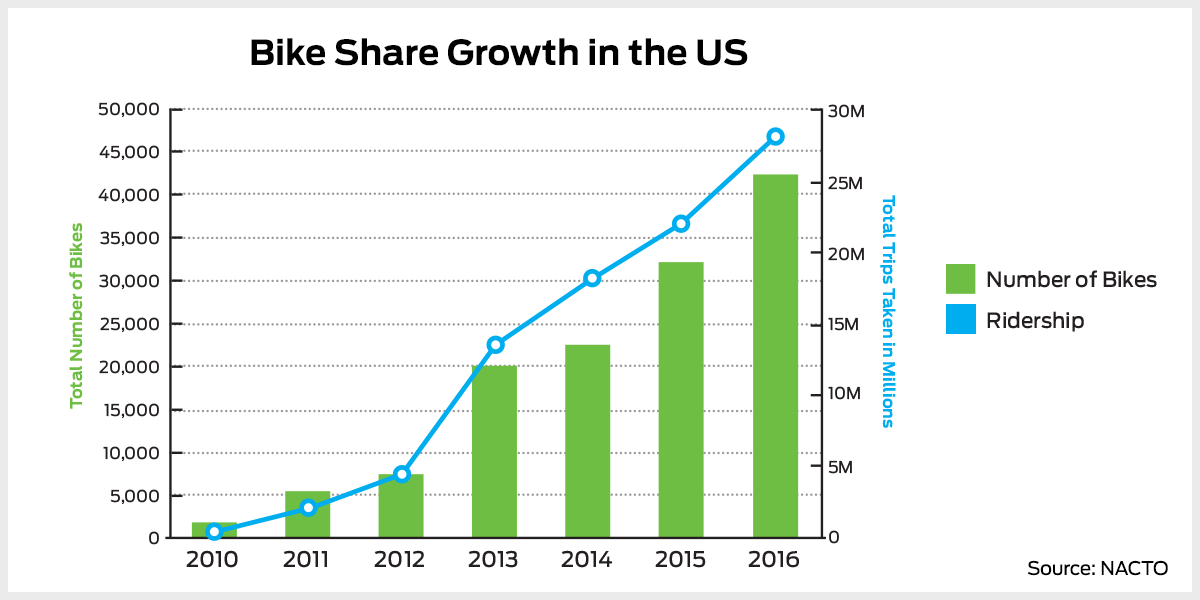
\includegraphics[width=0.4\textwidth]{intro}
  \caption{Bike Share Growth in the US}
  \label{fig_intro}
  \end{figure}

  \par In this project, we obtained the primary dataset provided by Citibike System Data. The data generated by these bike share systems are consisted of duration of travel, start time and date, stop time and date, start station name, stop station name, station ID, station latitude and lonitude, bike ID, user type(Customer = 24-hour pass or 3-day pass user; Subscriber = Annual Member), user gender and user's year of birth. Given adequate data from Jul 2013 to Sep 2017, we used data in 2016 year round. In our analysis, we attempt to evaluate the importance of different features and extract the non-trivial ones to create a prediction model for this problem. We then compare performances of different models and discuss their effectiveness and shortcomings. In this assignment, We mainly use the method of multiple linear regression analysis, Random Forest and XGBoost to forecast the bike share trip duration in New York City. An ensemble of Random Forest and XGBoost is also applied in this report. We evaluate these models based on the Fraction of Variance Unexplained (FVU). 

\section{Data}
  \par We obtain the data from the data system of Citi Bike, which is the national largest bike share program, with 10,000 bikes and 600 stations across Manhattan, Brooklyn, Queens and Jersey City\cite{bike}. It consists of data from the program's launch date, from 07/2013 to 09/2017. The dataset provided information is as shown in Table \ref{tab_1}. 
	\begin{center}
	\begin{table}[h!]
	\begin{tabular}{ |c|c| } 
	 \hline
	 Variate & Format \\ 
	 \hline
	 Trip Duration & in seconds format \\ 
	 \hline
	 Start Time and Date & Timestamp\\ 
	 \hline
	 Stop Time and Date & Timestamp\\
	 \hline
	 Start Station Name & String\\
	 \hline
	 End Station Name & String\\
	 \hline
	 Station ID & Number\\
	 \hline
	 Station Lat/Long & Number\\
	 \hline
	 Bike ID & Number\\
	 \hline
	 User Type & Customer or Subscriber \footnote{Customer = 24-hour pass or 3-day pass user; Subscriber = Annual Member} \\
	 \hline
	 Gender & Number \footnote{0=unknown; 1=male; 2=female} \\
	 \hline
	 Year of Birth & Number\\
	 \hline
	\end{tabular}
	\caption{Dataset Variable and Type}
	\label{tab_1}
	\end{table}
	\end{center}
	Basically, there were [XXXX] bike stations and total number of rides in dataset is [XXXXX]. Total number of customers' rides is [XXXXX] and subscribers' rides is [XXXX].

Before choosing useful features, we do some cleaning work since there are some deficient data in the dataset: some rides miss parts of the users’ information such as the age and sex; also by looking at the start time and stop time fields, we find some rides take over 1 million seconds, roughly around one month, which is unreasonable. Besides, we calculated the speed of each ride and find that some speeds are too low or too high. To avoid the effect of these outliers, we restricted the speed of each ride to be greater than 1 m/s and less than 8.5 m/s, which falls in the range between the speed of walking and driving. 

After the cleaning process, we randomly choose 30,000 data from each month of the 2016 to form our dataset with size 360,000 in total. And we split it into three sets: training, validation and test, each with 120,000 rides.


\section{Predictive Task}

\section{Models and Methodology}

\section{Literature}

\section{Results and Conclusions}

% The \textit{proceedings} are the records of a conference.\footnote{This
  % is a footnote}
% \subsection{Type Changes and {\itshape Special} Characters}

% \subsection{Math Equations}

% \subsubsection{Inline (In-text) Equations}

% \begin{table}
%   \caption{Frequency of Special Characters}
%   \label{tab:freq}
%   \begin{tabular}{ccl}
%     \toprule
%     Non-English or Math&Frequency&Comments\\
%     \midrule
%     \O & 1 in 1,000& For Swedish names\\
%     $\pi$ & 1 in 5& Common in math\\
%     \$ & 4 in 5 & Used in business\\
%     $\Psi^2_1$ & 1 in 40,000& Unexplained usage\\
%   \bottomrule
% \end{tabular}
% \end{table}



% \begin{table*}
%   \caption{Some Typical Commands}
%   \label{tab:commands}
%   \begin{tabular}{ccl}
%     \toprule
%     Command &A Number & Comments\\
%     \midrule
%     \texttt{{\char'134}author} & 100& Author \\
%     \texttt{{\char'134}table}& 300 & For tables\\
%     \texttt{{\char'134}table*}& 400& For wider tables\\
%     \bottomrule
%   \end{tabular}
% \end{table*}
% % end the environment with {table*}, NOTE not {table}!

% It is strongly recommended to use the package 
% and follow its main principles of typography with respect to tables:
% \begin{enumerate}
% \item Never, ever use vertical rules.
% \item Never use double rules.
% \end{enumerate}
% It is also a good dingsidea not to overuse horizontal 


% \subsection{Figures}


% \begin{figure}
% 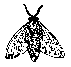
\includegraphics{fly}
% \caption{A sample black and white graphic.}
% \end{figure}

% \begin{figure}
% 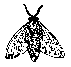
\includegraphics[height=1in, width=1in]{fly}
% \caption{A sample black and white graphic
% that has been resized with the \texttt{includegraphics} command.}
% \end{figure}



% \begin{figure*}
% 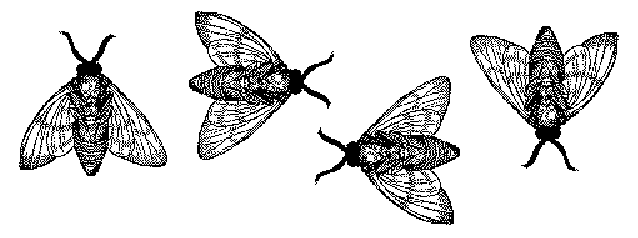
\includegraphics{flies}
% \caption{A sample black and white graphic
% that needs to span two columns of text.}
% \end{figure*}


% \begin{figure}
% 
\includegraphics[height=1in, width=1in]{rosette}
% \caption{A sample black and white graphic that has
% been resized with the \texttt{includegraphics} command.}
% \end{figure}


% \end{document}  % This is where a 'short' article might terminate

